 %!TEX root = main.tex
\chapter{Membraneless organelles and liquid-liquid phase transitions}


Major organelles in cells, e.g.~the nucleus, the ER, or mitochondria, are enclosed by membranes.
Transport between compartments is controlled by pores and channels.
This is not true for all organelles: structures like nucleoli and similar blobs in the cytosol seem to be well defined three dimensional structures without an enclosing membrane.
Over that last ten years, scientists have started to characterize such structures and discovered that these structures are essentially \emph{droplets} of one liquid embedded in another liquid (the cytosol) \citet{brangwynne_germline_2009}.

Among the earliest known examples of membraneless organelles are nucleoli can Cajal bodies.
Nucleoli were first described in the early 19th century.
Subsequently, it was shown that nucleoli are the structures in which ribosomal RNAs are transcribed.
They form seemingly homogeneous structures with a markedly different protein and RNA composition than the surrounding nucleus without being enclosed by a membrane.
Cajal bodies were first described by Santiago Ramon y Cajal.
They are often associated with nucleoli and seem to be involved in various steps of RNA processing.
There exact function is not well described.

Cytosolic membraneless structures include stress granules, P-bodies, or P-granules.
These granules form in particular developmental stages or specific environmental conditions.
Most fundamental discoveries about the nature of such membraneless organelles have been made with P-granules which are important in early C.~elegans development.
P-granule stands for ``perinuclear RNA-rich cytoplasmic granule''.
They are mixtures of RNA and RNA-binding-proteins many of which are implicated in translational control (possibly due to their P-granule association.)
In their seminal paper, \citet{brangwynne_germline_2009} show that these P-granules behave like liquid droplets immersed in the cytosol and that condensation and dissolution of these droplets are governed by physical principles of phase transitions.
Biology seems to exploit these principles to achieve an efficient separation of protein and mRNA between two daughter cells of the first cell division in C.~elegans development.
Such liquid-liquid phases transitions have since been discovered in many cell biological contexts.
While their precise role often remains elusive, it by now seems clear that such condensates and phase transitions are an important facet of organization in cells.


\section{Phase transitions}
Phases and phase transitions are part of our day-to-day experiences: water freezes and boils, oil and water don't mix, eggs become hard as you boil them.
Fig.~\ref{fig:h2o_phases} shows a simplified phase diagram of water with the solid (ice), liquid (water), and gaseous (vapor) phases.

The part of the phase diagram that will be of greatest interest here is the boundary between the liquid and the vapor phase.
This boundary has a sudden end in a critical point.
Have a look at the video \href{https://youtu.be/-AXJISFdC2E}{youtu.be/-AXJISFdC2E}, which shows the behavior of a substance in the vicinity of the critical point.
Below the critical point, the system can coexist in two phases.
As one approaches the critical point, the density of gas and vapor become more similar until at the critical point the differences between the two phases disappears.
Above the critical point, the substance is homogeneous -- a state known in super-critical liquid.

The aspect of the phase diagram that is most relevant for our discussion below in that of condensation: Consider a system in the vapor phase. As you begin to cool down the system, vapor at some point becomes super-saturated and it condenses into droplets (fog).
This condensation corresponds to approaching the boundary between the liquid phase and vapor phase horizontally.

\begin{figure}[tb]
	\centering
	\includegraphics[width=0.8\textwidth]{figures/Phase_diagram_of_water_simplified.png}
	\caption{Simplified phase diagram of water as a function of temperature and pressure. Ambient pressure is indicated by a horizontal line, 0$^\circ$C and $100^{\circ}$C are indicated by horizontal lines.}
	\label{fig:h2o_phases}
\end{figure}


\subsection*{Phases of multicomponent systems}
The discussion above used water as an example.
Water has a rich phase diagram, but this example has one fundamental limitation: nothing else but $\mathrm{H_2 O}$.
All systems we will encounter in biology are complicated mixtures of many different types of molecules that can interact in myriad ways.
From thermodynamics, you should be familiar with Gibb's phase rule:
\begin{equation}
	f = c - p + 2
\end{equation}
Here, $f$ is the number of degrees of freedom, $c$ is the number of components, and $p$ is the number of co-existing phases.
It immediately follows that systems composed of many different molecular species ($c$) can co-exist in many different phases $p$.
At co-existence, these phases share the same temperature and pressure, but differ in composition of the different species.
The relative amount of each phase and its composition adjusts such that the chemical potential of each compound is equal in each phase.
These compositions can either be almost completely pure species (like oil and water mixtures) or more even mixtures (like 30/70).
The closer the system is to a critical point, the more even the mixtures are.
Whether a multi-component system separates into several phases depends not only on the temperature, pressure and the composition of the system.


\section{Multi-component systems}

\subsection*{Entropy and energy mixtures}
The phase separation, or de-mixing, is driven by conflicting entropy and energetic (enthalpic) tendencies.
The energy of the system is minimized by placing molecules that interact  favorably with each other next to each other.
Entropy, on the other hand, is maximized by randomly distributing the species in space resulting in one homogeneous phase.
We will now explore these competing tendencies in a simple toy model of a solution of a self-interacting species in a solvent, see Fig.~\ref{fig:multi_component_mixtures}.

\begin{figure}[tb]
	\centering
	\includegraphics[width=0.7\textwidth]{figures/Brangwynne_interactions.png}
	\caption{Illustration of multi-component mixtures. From \citet{brangwynne_polymer_2015}.}
	\label{fig:multi_component_mixtures}
\end{figure}

The white balls in Fig.~\ref{fig:multi_component_mixtures} represent the solvent, the green balls the protein or polymer whose condensation we are interested in (we'll call it protein for simplicity).
The interaction energy can be written as the number of contacts between solvent molecules $u_{ss}$, between solvent and protein $u_{sp}$, and between proteins $u_{pp}$.
The total energy of the mixture is therefore given by
\begin{equation}
	U = n_{ss}u_{ss} + n_{sp}u_{sp} + n_{pp}u_{pp}
\end{equation}
where $n_{ss}$, $n_{sp}$, and $n_{pp}$ are the number of times the respective neighbor relations are observed.

While we will never be able to enumerate the exact number of neighbor relations, we can readily estimate the expected number of contacts.
The typical number of contacts one solvent molecule makes is called the coordination number $z$.
For simplicity, lets assume that monomers have similar size as solvent molecules and arrange them on a lattice.
If the state of the systems is a random mix with monomer fraction $\phi$, the energy of the system is
\begin{equation}
\begin{split}
U &= \frac{N z}{2} \left[(1-\phi)^2 u_{ss} + \phi^2 u_{pp} + 2\phi(1-\phi)u_{sp}\right] \\
&= \frac{N z}{2}\left[\phi(1-\phi)(2u_{sp} - u_{pp}-u_{ss}) + \phi(u_{pp}-u_{ss}) + u_{ss}\right]
\end{split}
\end{equation}
The term proportional to $\phi(1-\phi)$ is the contribution of contacts between the types, while the term proportional to $\phi$ is simple the difference between the pure types.
The take home here is that as a function of concentration $\phi$, the enthalpy is a parabola that can either have positive curvature favoring mixtures or negative curvature favoring demixing.

Demixing is opposed by entropy: many energetically unfavorable states can have more weight than few favorable states.
Entropy is the logarithm of the number states available given the constraints.
Consider a lattice model of the solution and ignore for a moment that the monomers of the polymer are strung together.
In a random mixture, we can pick for each lattice site independently whether its solvent or monomer.
This results in
\begin{equation}
e^{(S+c)/k} = \frac{N!}{(N\phi)!(N(1-\phi))!}
\end{equation}
configurations (where $k$ is Boltzmann's constant).
The logarithm of this number is the entropy (up to an additive constant).
To calculate its magnitude, we use the well known Stirling's approximation for factorials $\log n! \approx n\log n - n$ and find
\begin{equation}
\begin{split}
S + c &= kN\left[\log N - \phi\log(\phi N) - (1-\phi)\log((1-\phi)N)\right] \\
& = -N(\phi\log(\phi) + (1-\phi)\log(1-\phi))
\end{split}
\end{equation}
Combining the interaction energy with the mixing entropy, we arrive at the free energy $F=U-TS$ of the idealized system (assuming $u_{pp}=u_{ss}$ and dropping constants):
\begin{equation}
\frac{F}{N} =  \phi(1-\phi) \frac{z(2u_{sp} - u_{pp}-u_{ss})}{2} + kT\left[\phi\log(\phi) + (1-\phi)\log(1-\phi)\right]
\end{equation}
Whether the solution will spontaneously separate into a phase of high and low concentration of the protein, depends on whether the free energy of the homogeneous mixed system is lower than the sum of the energies of two systems at high/low monomer concentration.


\subsection*{Instability of a mixture}
Consider a homogeneous mixture with monomer concentration $\phi$ and compare this to a two phase mixture in which one phase (fraction $\alpha$) has concentration $\phi_1$ and the other phase (fraction $1-\alpha$) has concentration $\phi_2$.
To conserve mass $\alpha \phi_1 + (1-\alpha)\phi_2 = \phi$.
Under what conditions will a mixture of two phases will have lower energy than the homogeneous case?

The stability of a configuration depends on the curvature of the free energy in $\phi$.
This is illustrated in Fig.~\ref{fig:unstable_mix}.
The free energy of a mixture with fraction $\alpha$ lies on a straight line connecting the two pure phases with concentrations $\phi_{1/2}$.
Conservation of mass requires that the average concentration doesn't change, hence the relevant comparisons are all on a vertical line.
This considerations immediately tells us that a mixture is stable if the free energy is convex, i.e., the curvature is positive.
Otherwise, it is always possible to lower the free energy by splitting the solution into a mix of two phases.

\begin{figure}[tb]
	\centering
	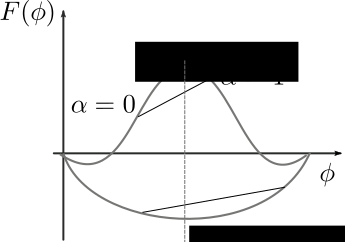
\includegraphics[width=0.6\textwidth]{unstable_mix.png}
	\caption{Unstable mixture}
	\label{fig:unstable_mix}
\end{figure}

\subsection*{Surface tension}
Phase separation happens when like interactions are sufficiently strong to overcome entropy favoring mixing.
At the surfaces of two phases, however, molecules enjoy a smaller number of like interactions than in the bulk of the either phase.
Hence surfaces between phases are associated with a free energy cost.
This cost results in a tendency to minimize the surface area given the volume and the optimal geometry is obviously a sphere.
Effectively, the surface is under tension driving shapes towards the lowest free energy geometry.
Surface tension has units energy/area or Newton/length.

When three different phases (or a solid, a liquid and a gas) meet, the three phase interface depends on the relative surface tensions associated with the three interfaces.
The resulting behavior and contact angles can be calculated from the balance of forces at the contact line.

\subsection*{Nucleation}
A homogeneous solution can get super-saturated.
Super-saturation refers to a state where the system should have separated into two phases, but this separation hasn't happened yet.
Such delayed condensation can occur since the forming small droplets can be energetically disfavorable even though the equilibrium state would favor phase separation.
This phenomenon is known from our atmosphere: It is possible to ``seed'' clouds with small particles to produce rain.
These small particles act as nuclei around which rain drops can form -- a process energetically more favorably than drop formation without a nucleus.

The energetic barrier for nucleating a droplet can be understood by a simple argument involving the scaling of the surface and the bulk of a droplet.
The relative contributions of free energy of the bulk and surface depend on the size of the droplet.
For a spherical droplet, the free energy will scale with the radius as
\begin{equation}
G(r) = -\alpha r^3 + \beta r^2
\end{equation}
where $\alpha,\beta$ are positive constant with the appropriate dimensions.
At very small $r$, the free energy increases with $r$ and small droplets are unstable.
Only above the nucleation radius $r^* = \frac{2\beta}{3\alpha}$ do droplets grow deterministically.
This phenomenon is known as nucleation.
One common every day example were nucleation can be observed is the instant freezing of super-cooled water.
Have a look at this video \href{https://youtu.be/PM9nwYF1uR4}{youtu.be/PM9nwYF1uR4}.


\section{Condensates in biology}

\subsection*{Droplets are often RNA-protein mixtures}
To drive phase separation and form droplets, the constituents need to be able to form multivalent interactions.
Obviously, 1-1 interactions can't form higher order structures, only dimers.
Similarly, if each molecule can only interact with two other molecules, one can form polymer chains by no extended 3D structures.
Instead, at least 3-valent at better still multi-valent interactions are necessary to drive phase transitions.
In the lattice example above, the multi-valency was given by the number of neighbors on the lattice.
In droplets in the cytosol, such multivalent interactions are mediated by intrinsically disordered regions of proteins that often contain repetitive linear motives that interact with each other or RNA.
These regions are also called low complexity regions due to their repetitive sequence and biased amino acid composition.
Fig.~\ref{fig:mol_interactions} shows several such low complexity regions in different proteins along with the types of interactions they generate.

\begin{figure}[tb]
	\centering
	\includegraphics[width=\textwidth]{figures/Brangwynne_molecular_basis.png}
	\caption{Modes of multivalent interactions in different types of cytosolic droplets. Figure from \citet{brangwynne_polymer_2015}.}
	\label{fig:mol_interactions}
\end{figure}

Similarly, interactions between RNA and proteins can generate droplets: RNA can serve as a scaffold that is cross-linked many times by proteins (or protein complexes) that have at least 2 RNA binding domains.

\subsection*{P granules in {\it C.~elegans}}
The notion that membraneless organelles might be essentially liquid droplets embedded in the cytosol was put forward in a publication in 2009 by \citet{brangwynne_germline_2009}.
P-granules are protein-RNA assemblies that are involved in the determination of cell fate in the early {\it C.~elegans} embryo, see Fig.~\ref{fig:pgranules}.
Initially, P-granules are distributed across the embryo and appear and dissolve in a spatially homogeneous fashion.
They move around by cytoplasmic flow.
This flow does in fact transport as many P-granules left as it does right.
Nevertheless, P-granules concentrate at the posterior end.
This concentration is caused by different conditions in the anterior and posterior ends: Droplets dissolve at the anterior end and form at the posterior end.
This effectively introduces a sink which concentrates the droplets in one of the daughter cells.

\begin{figure}[tb]
	\centering
	\includegraphics[width=\textwidth]{figures/Brangwynne_Pgranules_intro.png}
	\caption{P-granules in {\it C.~elegans} embryos. Figure from \citep{brangwynne_germline_2009}.}
	\label{fig:pgranules}
\end{figure}

These droplets are remarkably dynamic.
Photobleaching of fluorescently labeled droplet components shows that components rapidly diffuse across the droplet and also move between the cytosol and the droplet.
When sheared, P-granules flow, drip, and wet just like liquids.


\begin{figure}[tb]
	\centering
	\includegraphics[width=\textwidth]{figures/Brangwynne_Pgranules_liquid.png}
	\caption{P-granules behave like liquids that rapidly exchange material with the surrounding cytosol. Figure from \citep{brangwynne_germline_2009}.}
	\label{fig:pgranules_liquid}
\end{figure}

\subsection*{Putative functional roles of condensates}
The function of membraneless organelles continues to be poorly characterized, but several plausible hypotheses exist:
\begin{itemize}
	\item {\it micro-reactors}: Droplets are greatly enriched for particular sets of proteins and RNAs. Hence specific reactions between these components are expected to be much faster in such droplets compared their speed if components were randomly distributed in the cytosol.
	\item {\it garbage dumps}: uncontrolled protein aggregation is dangerous. Hence droplets could represent a controlled way to absorb excess material that would otherwise be prone to uncontrolled aggregation. Similar, the droplets could serve to sequester harmful (damaged, misfolded, etc) proteins.
	\item {\it storage:} Membraneless organelles could be used for RNA storage that would be ready for transcription and/or modification when the conditions change.
\end{itemize}
As more research is done, the roles of droplets will become better defined and more roles will likely be discovered.
Compartmentalization plays an important role at many scales of biological organization and there is every reason to believe that biology exploits the potential of membraneless organelles.